\subsection{Kepler’s Second Law: When Area Became the Clock of the Cosmos}

Before Kepler, area was something you calculated after the fact—like the size of a field or the footprint of a cathedral. But Kepler had a more radical thought: \textbf{What if area could measure time? What if the orbit of a planet swept space with a kind of rhythm?}

Kepler’s Second Law, as stated in \textit{Astronomia Nova} (1609), can be understood like this:

\begin{quote}
A planet doesn’t sweep through equal amounts of space in equal amounts of time. Instead, it sweeps through \textbf{equal areas} in equal times.
\end{quote}

This means: when a planet is \textit{closer to the Sun}, it \textit{moves faster}, and when it’s \textit{farther from the Sun}, it \textit{slows down} — but always in such a way that the imaginary line from the Sun to the planet sweeps out equal areas in equal time intervals.

Visually, it’s as if the Sun is tethered to the planet with an invisible rope, and that rope sweeps across wedges of space that are always the same size if you wait the same amount of time — no matter where the planet is in its orbit.

This was radically different from earlier beliefs that planets moved in perfect circles at constant speeds. Kepler’s insight was that \textbf{motion itself is dynamic and changing}, tied directly to the planet’s distance from the Sun.

\begin{figure}[H]
\centering
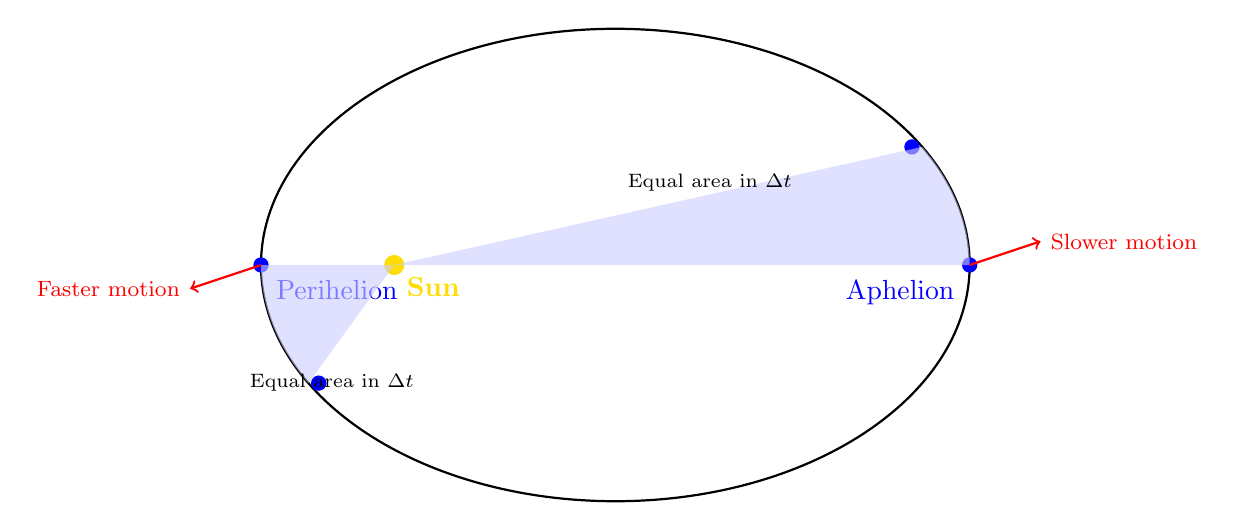
\begin{tikzpicture}[scale=3]

  % Sun focus offset (a = 1.5, b = 1)
  \def\c{0.936} 

  % Ellipse
  \draw[thick] (0,0) ellipse (1.5 and 1);

  % Sun at left focus
  \coordinate (Sun) at (-0.936, 0);
  \filldraw[yellow!80!orange] (Sun) circle (0.04) node[below right=1pt] {\textbf{Sun}};

  % Aphelion point
  \coordinate (Aphelion) at (1.5, 0);
  \filldraw[blue] (Aphelion) circle (0.03) node[below left=2pt] {Aphelion};

  % Perihelion point
  \coordinate (Perihelion) at (-1.5, 0);
  \filldraw[blue] (Perihelion) circle (0.03) node[below right=2pt] {Perihelion};

  % Additional planet positions
  \coordinate (A2) at ({1.45*cos(30)}, {1.0*sin(30)}); % near aphelion
  \coordinate (P2) at ({-1.45*cos(30)}, {-1.0*sin(30)}); % near perihelion
  \filldraw[blue] (A2) circle (0.03);
  \filldraw[blue] (P2) circle (0.03);

  % Area near aphelion (slower)
  \fill[blue!20, opacity=0.6]
    (Sun) -- (Aphelion) arc[start angle=0, end angle=30, x radius=1.5cm, y radius=1cm] -- cycle;

  % Area near perihelion (faster)
  \fill[blue!20, opacity=0.6]
    (Sun) -- (Perihelion) arc[start angle=180, end angle=210, x radius=1.5cm, y radius=1cm] -- cycle;

  % Arrows for velocity
  \draw[->, thick, red] (Aphelion) -- ++(0.3,0.1) node[right] {\footnotesize Slower motion};
  \draw[->, thick, red] (Perihelion) -- ++(-0.3,-0.1) node[left] {\footnotesize Faster motion};

  % Area labels
  \node at (0.4,0.35) {\scriptsize Equal area in $\Delta t$};
  \node at (-1.2,-0.5) {\scriptsize Equal area in $\Delta t$};

\end{tikzpicture}
\caption{Kepler’s Second Law: Equal areas swept in equal times—even when speeds vary}
\end{figure}

\subsubsection{The History and Drama Behind \textit{Astronomia Nova}}

Johannes Kepler published \textit{Astronomia Nova} in 1609, after nearly a decade of intense work trying to make sense of the observational data gathered by Tycho Brahe — especially for the planet Mars.

Kepler began with a belief in perfect cosmic harmony — circular orbits, Platonic solids, mystical geometry. He was a deeply religious man who thought that to study the heavens was to understand the mind of God.

When Tycho Brahe offered him access to the most precise astronomical data of the time, Kepler hoped to confirm the harmony he envisioned. But instead, the data refused to cooperate.

\subsubsection{The 8-Minute Error}

Kepler spent years trying to model Mars’s orbit using circular paths and epicycles, but there was always an \textbf{8-minute discrepancy} that wouldn’t go away. Rather than ignore or fudge the data, Kepler considered it a sign that his entire model needed to be rethought.

That small inconsistency led to a massive revelation.

\subsubsection{Kepler’s Breakthrough}

Kepler ultimately discovered that Mars moved in an \textbf{elliptical orbit}, not a circular one. This led to two major laws, both introduced in \textit{Astronomia Nova}:

\begin{itemize}
  \item \textbf{First Law:} Planets move in ellipses, with the Sun at one focus.
  \item \textbf{Second Law:} A planet sweeps out equal areas in equal times.
\end{itemize}

The book itself reads like a dramatic chronicle of Kepler’s intellectual struggle. It’s filled with calculations, digressions, metaphysical reflections, and deep frustration — an almost confessional record of scientific obsession.

\subsubsection{Why Did Kepler Write It?}

\begin{itemize}
  \item \textbf{Scientific:} He wanted to uncover the real structure of the cosmos, not just make predictive models.
  \item \textbf{Philosophical/Religious:} Kepler saw mathematics as the divine language through which God designed the universe. To him, discovering the laws of planetary motion was an act of worship.
  \item \textbf{Personal:} He was driven by conviction, obsession, and the belief that he had a sacred calling to reveal cosmic truth.
\end{itemize}


\begin{quote}
``I am stealing the golden vessels of the Egyptians to build a tabernacle to my God... If you forgive me, I shall rejoice; if you are angry, I shall bear it.''
— Johannes Kepler, justifying his use of pagan mathematics for holy insight.
\end{quote}

\begin{tcolorbox}[title=Kepler and the Singing Sun, colback=gray!5, colframe=black, fonttitle=\bfseries]

  \textbf{If Copernicus gave the Sun a throne, Kepler gave it a voice.}
  
  While Copernicus placed the Sun at the center of the cosmos for reasons of symmetry and elegance, \textbf{Johannes Kepler} went further: he made the Sun the \textit{engine} of celestial motion.
  
  Drawing from Pythagorean and Neoplatonic traditions, Kepler believed the planets moved in harmonious orbits not merely by geometry, but by a physical force radiating from the Sun—what he called a \textbf{"motive soul"}.
  
  This wasn’t metaphor. In his magnum opus, \textit{Harmonices Mundi} (The Harmony of the World), Kepler proposed that each planet’s motion traced a kind of \textbf{celestial music}, forming chords and scales as they orbited. Venus sang soprano, Jupiter droned bass.
  
  To Kepler, astronomy wasn’t just a science—it was a divine composition, and the Sun was both conductor and source.
  
  \begin{quote}
  \textit{“The Sun, not undeservedly, is called the lantern of the universe... the source of heat, the cause of motion.”} \\
  — \textbf{Johannes Kepler}
  \end{quote}
  
\end{tcolorbox}
  







\subsection{The Geometry Kepler Used (With a Bit of Archimedes)}

Kepler didn’t have calculus—but he had Archimedes.

To reason about planetary motion, Kepler sliced up orbits into tiny wedges—each bounded by the planet’s path, the Sun, and the line connecting the two. For small wedges over short times \( \Delta t \), the area is approximately:

\[
\text{Area} \approx \frac{1}{2} r^2 \Delta\theta
\]

Kepler argued: if this area is the same in every equal time slice, then the planet must move faster when it is closer to the Sun, and slower when farther away. It was a law not of speed, but of \textbf{sweeping}.

\[
r^2 \Delta\theta \propto \Delta t
\]

Kepler was effectively using **geometric exhaustion**—a technique borrowed from Archimedes—to discover a continuous principle from discrete slices.

\begin{quote}
\textit{“The radius vector describes equal areas in equal times.”}
\end{quote}

This wasn’t a metaphor. It was Kepler’s **clock**. His definition of time was not seconds on a dial, but the **geometry of space swept by planets**.

In doing so, he didn’t just discover a law of planetary motion—  
He redefined what it meant to move in the heavens.

\begin{tcolorbox}[colback=gray!5, colframe=black, title=\textbf{Historical Sidebar: Kepler’s Firmament as a Harmonic Horizon}, fonttitle=\bfseries, arc=1.5mm, boxrule=0.4pt]

  When Kepler rejected the old crystalline spheres, he didn’t discard the firmament’s significance—he reimagined it.
  
  For medieval cosmology, the firmament was a solid, rotating sphere carrying the fixed stars. For Kepler, it became something subtler: the **outer boundary of a cosmic harmony**, a geometric stage where God’s design was displayed.
  
  In his \textit{Harmonices Mundi} (1619), Kepler argued that planetary motions formed a celestial music—an audible harmony encoded in the ratios of their speeds and distances. The firmament, once thought a physical shell, now marked the **limit of this divine symphony**.
  
  \medskip
  
  \textbf{In Kepler’s universe:}
  
  \begin{itemize}
    \item The firmament was no longer a mechanical sphere, but a **mathematical coordinate**, a horizon of intelligibility.
    \item Geometry wasn’t just a tool for measurement—it was a window into the **mind of God**, who created the cosmos according to mathematical laws.
    \item The fixed stars weren’t just lights—they were the **outermost choir of creation**, framing the geometry of the planets’ paths.
  \end{itemize}
  
  By measuring the planets’ areas swept in time, Kepler wasn’t just solving a geometric puzzle. He believed he was deciphering **the rhythm of divine architecture**, written in the language of geometry.
  
  \begin{center}
  \emph{For Kepler, every orbit traced a hymn. Every triangle whispered a secret of the Creator.}
  \end{center}
  
\end{tcolorbox}
